\documentclass[12pt,a5]{bxjsarticle}

\usepackage{xltxtra}
\setmainfont{IPAPMincho}
\setsansfont{IPAPGothic}
\setmonofont{IPAGothic}
\XeTeXlinebreaklocale "ja"

\usepackage{hyperref}
\usepackage{listings}
\usepackage{verbatim}
\usepackage{amsmath}

\newcommand{\e}{\mathrm{e}}

\title{物理学情報処理論2 problem12}
\date{}

\begin{document}
\maketitle

\section{}

\[
  \begin{cases}
    \frac{dx}{dt} = a - (b + 1) x + x^2 y \\
    \frac{dy}{dt} = bx - x^2 y
  \end{cases}
\]
について考える。
これは生体内で、周期性を作ったり、情報を保持したりする機構をモデル化した、
ブリュッセレーターと呼ばれる微分方程式である。
これを$ a = 1 $、$ b = 0.3, 1.9, 2, 2.1, 2.5 $で数値的にSymplectic法で解いたものが以下のグラフである。

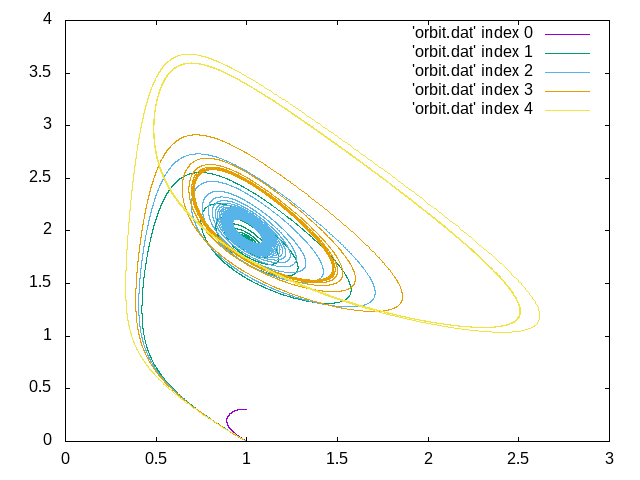
\includegraphics[width=\linewidth]{orbit.png}

$ a = 1 $の場合、$ b = 2 $に振舞いの変わる境が存在し、
それ以下の場合には特定の値へと渦を描きつつ収束していく。
それより大きな場合には、特定の領域を周回しつつも収束はしない(振動する)。
ということが知られている。

解析的な振舞いを調べたことはあったが、
実際に解がどのような線を動くのかを見たことがなかったため、図示できて良かった。

\section{}
講義の感想

物理的な問題について、専門ではなくその物理現象について理解をしていないこともあったが、
サンプルのグラフなどによる説明によりその発展を計算することが、できて良かったと思います。

以下のスクリプトを用いて、orbit.datから図を生成した。
\lstinputlisting[caption=plot.sh,language=bash]{plot.sh}

\end{document}
